\newpage
\subsection{Miscellaneous}
The whole project code and the PCB design can be accessed via the corresponding links in section \ref{sec:references}.

\subsubsection{Switching between measurement modes (code description)}
\label{sec:method_switch_code}
At the beginning of our project, we thought of a couple of switching methods. One of our ideas was to use multiple buttons, one for each measurement type. This method would make up for a simpler code implementation but would require a tremendous amount of pins on the MCU. Due to this drawback, we opted out of this method. Another method we discussed was the use of a rotary encoder, but in the end, we opted to use just two buttons, as a means of switching through the measurement modes in a menu-like way. The buttons are used to switch to the previous or the next measurement type, respectively. This way, we only use two pins, and could easily extend the types of measurement, without changing the front end of the code. The two buttons are connected between two IRQ pins of the MCU and ground. The internal pull-up resistors of the two pins are activated in code, this way there is never an unknown state at the used pins, which could trigger a false switch. The whole switching methodology relies on the use of interrupts, rather than the often-used polling method. The two ISRs, which are being called at a triggered interrupt, are one-line functions, flipping either the "next" or "prev" boolean variables to true. Using the Arduino framework's \textit{attachInterrupt} function, these ISRs are attached to their matching IRQ pins, specified to trigger an interrupt only at a falling edge, i.e. when the logic level at the input goes from HIGH to LOW. In the main loop, these two variables are checked whether they are true, in which case another variable, "mode select", is incremented or decremented. At every interrupt detection, a delay of approximately 170 milliseconds is used to counter the buttons' rapid on-off clicking, which is due to mechanical contact and imperfections in the buttons' construction. Based on the "mode select" variable, the specific measurement mode functions are then selected in a switch statement. During this time, the specific relay combination is selected as well, within the function called \textit{selectRelayCombination}, based on section \ref{sec:method_safety_relays}.

\subsubsection{Battery level indicator}
\label{sec:method_bat_indicator}
The ability to alert the user to change the battery is a crucial one, especially in a device like a multimeter. For this reason, we wanted to include some sort of alerting system in our device, too. As the MCU is powered through an LM7805 linear voltage regulator IC, so we chose the minimum adequate voltage level based on its datasheet. The datasheet states that the minimum input voltage required to maintain line regulation is 7.5V, so we chose this value as well. The voltage of the battery is read using an ADC pin and a voltage-divider of two identical, 100k$\Omega$ resistors. As the voltage-divider in this configuration will always output half of the supply voltage (in our case the voltage level of the battery), the specified minimum voltage level used in the code is also halved, i.e. 3.75V. At every measurement mode switching, a battery voltage level test takes place. If the supply voltage is below the specified threshold, an alerting message will appear on the fourth line of the LCD. This alert will not render the device unusable, it is there just to alert the user, as intended.

\subsubsection{Safety and mode switching}
\label{sec:method_safety_relays}
Our multimeter comes with safety measures for each of our modes. These are:
\begin{itemize}
    \item Voltage:      Built-in protection diodes in the buffer op-amp. (Up to 5mA)
    \item Current:      A 5A fuse and temperature shut-off built-in
    \item Resistance:   Diode to prevent outside voltage from interacting with the analogue pin
    \item Frequency:    Capacitor to interrupt DC-voltage and a zener-diode to prevent a voltage over 5V
\end{itemize}

\begin{figure}[h]
    \centering
    \frame{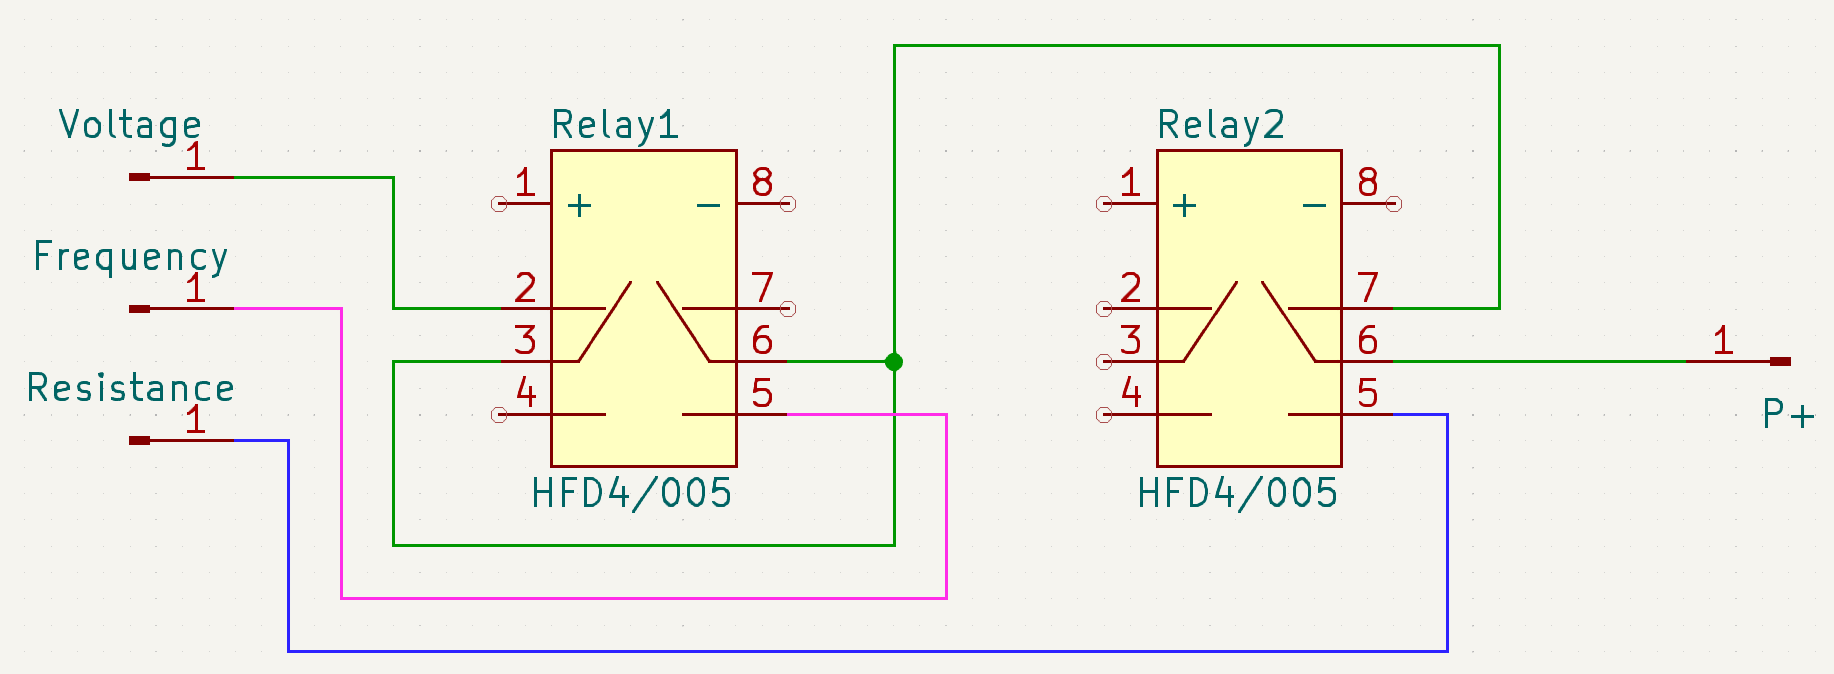
\includegraphics[width=1\linewidth]{images/RelayMat.png}}
    \caption{Relay-matrix principle}
    \label{fig:relmat}
\end{figure}

\noindent The method we used to switch between our modes was via two signal relays. This principle is shown in Figure \ref{fig:relmat} and the logic is:

\begin{itemize}
    \item Voltmeter mode: Relay1 \textcolor{red}{OFF} / Relay2 \textcolor{red}{OFF}
    \item Ohmmeter mode:  Relay1 \textcolor{red}{OFF} / Relay2 \textcolor{green}{ON}
    \item Frequency meter mode: Relay1 \textcolor{green}{ON} / Relay2 \textcolor{red}{OFF}
\end{itemize}

\noindent This makes sure that only one mode is connected to the probe input at a time, while the other ones are galvanic disconnected. The drawback then is the current draw derived from keeping the relays in the ON-state when using the ohmmeter and frequency meter.

\subsubsection{Project management}
Project management mainly involved creating the time plan which can be seen in the Appendix, distributing tasks to team members, setting up project infrastructure, and keeping the project on track. All of the decisions made were made with the consent of the majority of the team members. See Figure \ref{fig:TP} for a detailed plan of our project.

\subsubsection{Economy}
The whole project cost 1036.7 DKK. The bill of materials can be seen in section \ref{sec:appendix}, Appendix.